\subsection{Kühlbox}
\label{subsec:Kühlbox}

Damit die Getränke möglichst lange kühl bleiben, wurde eine Kühlbox aufgebaut. Dazu wurde der Bereich, welcher für die Flüssigkeiten bestimmt ist, mit Styropor ausgekleidet. Dieser hält die Kälte länger in der Box, da Styropor viele Luftblasen enthält und diese als gute Isolation dienen. Um den Effekt noch zu verstärken wurde Die Box zusätzlich mit Aluminiumtape verkleidet, was nochmals zusätzlich isoliert und auch die Box sauber verschliesst. Um die Getränke zusätzlich kühl halten zu können, wurde Platz für Kuhlakkus geschaffen, welche im Gefrierfach gefroren und dann bei Gebrauch zwischen den Flüssigkeiten platziert werden können. Dieser Aufbau ist in Abbildung \ref{fig:Kuehlbox} zu sehen.

\begin{figure}[H]
	\centering
	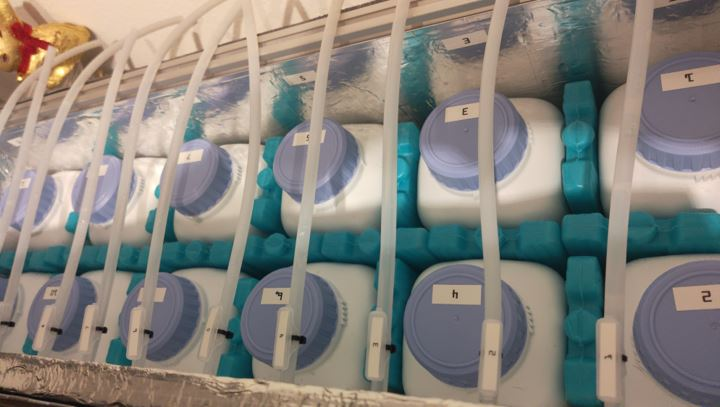
\includegraphics [width=0.8\textwidth]{graphics/Kuehlbox}
	\caption{Kühlbox des Partymixers}.
	\label{fig:Kuehlbox}
\end{figure} 

Cocktails werden normalerweise sehr kalt serviert. Dabei spricht man bei gerührten Cocktails von 2$^\circ$C - 4$^\circ$C und bei geschüttelten Cocktails von 0$^\circ$C - 2$^\circ$C. Diese Temperaturen werden mit Eis erreicht. Dieses muss beim PartyMixer separat hinzugefügt werden. Um jedoch die Getränke auch ohne Eis kalt geniessen zu können wurde das Ziel gesetzt, dass die Kühlbox die Getränke während mindestens 8std. kühl hält. Dies soll unter folgenden Bedingungen zu Hause erreicht werden können: \cite{mangomix_cocktail_2020}

\begin{itemize}
\item Vorherige Lagerung der Getränke im Kühlschrank bei 5$^\circ$C im unteren Bereich des Kühlschrankes
\item Einsetzen der gefrorenen Kühlakkus in die Maschine vor Gebrauch 
\item Betrieb der Maschine bei geschlossener Kühlbox
\end{itemize}

Diese Bedingungen können von jedem Benutzer eingehalten werden und sind somit für den Betrieb auch realistisch. Das Ziel war es, dass die Getränke in der Kühlbox über den Verlauf eines ganzen Abends von 18:00 Uhr bis 02:00 Uhr unter den vorhin genannten Bedingungen eine Temperatur von 5$^\circ$C nicht überschreiten. 

Um dies zu testen, wurde die Maschine unter den oben genannten Bedingungen einmal komplett befüllt und über eine Zeitdauer von 24std. ausgemessen. Die Raumtemperatur betrug dabei 22.6$^\circ$C. Die Flüssigkeitsbehälter wurden mit Wasser komplett befüllt und im Kühlschrank auf exakt 5$^\circ$C abgekühlt. Die Kühlelemente wurden im Gefrierfach gefroren. In Abbildung \ref{fig:Kaeltetest} ist das Ergebnis zu sehen.

\begin{figure}[H]
	\centering
	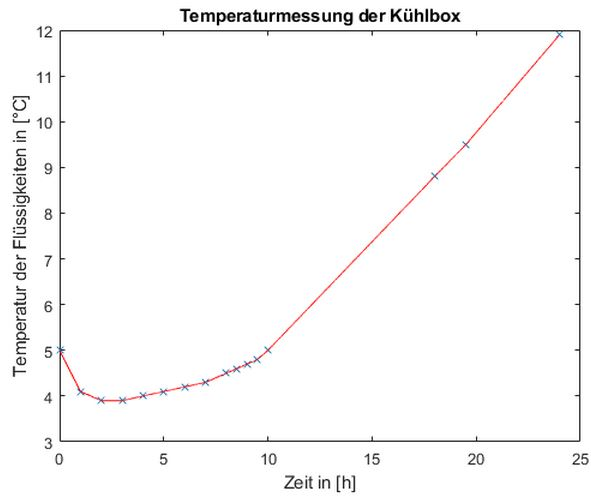
\includegraphics [width=0.8\textwidth]{graphics/Kaeltetest}
	\caption{Kältetest des Partymixers}.
	\label{fig:Kaeltetest}
\end{figure} 

Der Test hat gezeigt, dass die Flüssigkeiten sich durch die Kühlakkus zuerst wie erwartet noch ein wenig abkühlen, bevor die Temperatur wieder anfängt anzusteigen. Nach 8std. erreichten die Flüssigkeiten eine Temperatur von 4.6$^\circ$C und nach 10std. wurde die 5$^\circ$C Marke erreicht. Es können also unter den genannten Bedingungen über eine Zeitdauer von 10std. gekühlte Getränke aus der Maschine genossen werden, welche eine Temperatur von 4$^\circ$C - 5$^\circ$C haben.  




